\documentclass[11pt,a4paper]{article}
\usepackage[margin=2.5cm]{geometry}
\usepackage{amsmath,amssymb,booktabs,graphicx,natbib,hyperref,setspace}
\setstretch{1.1}
\title{Learning Marginal Effects for Goal Programming: Shrinkage-Adjusted Predict-then-Optimize Budget Allocation for Social Goals}
\author{Quang-Vinh Dang\\British University Vietnam, Hung Yen, Vietnam\\
\texttt{vinh.dq4@buv.edu.vn}\quad ORCID: 0000-0002-3877-8024}
\date{}
\begin{document}
\maketitle
\begin{abstract}
Public budgets are often allocated to attain several social goals at once, and goal programming (GP) is a standard way to do so. Its input, the marginal effect of spending on each goal, is rarely known and must be learned from historical data. We study a predict-then-optimize GP for budget allocation in which ridge regression estimates the effects and the GP is solved on the predictions. We add a simple adjustment that shrinks each predicted effect by $\lambda$ times its cross-validated residual standard deviation. In a controlled simulation with 60 decision units and four goals, we compare equal allocation, plug-in GP, shrunk GP, and an oracle with known effects, under Chebyshev and weighted-sum GP. Learning the effects removes most of the gap between equal allocation and the oracle. Under Chebyshev GP, worst-goal shortfall falls from about $0.47$ (equal split) to between $0.21$ and $0.25$, against an oracle value of about $0.14$. Shrinkage helps modestly for Chebyshev GP once training data are plentiful, by about $0.01$ in worst-goal shortfall at $\lambda\in[0.5,1]$ with $n=1000$. It worsens the worst-goal shortfall of weighted-sum GP at every setting we tried. All results are simulated; no field data are used.
\end{abstract}
\noindent\textbf{Keywords:} goal programming; multiple objective programming; machine learning; predict-then-optimize; public budget allocation; Chebyshev goal programming

\section{Introduction}
Goal programming \citep{charnes1961,ignizio1976,tamiz1998} lets a decision maker state aspiration levels for several objectives and then minimises unwanted deviations from them. It is widely applied in public policy and sustainable development \citep{romero1991}. A GP model needs technical coefficients that say how much each decision moves each goal. In budget allocation these are marginal effects of spending in each region or programme on health, education, employment and similar outcomes. They are not observed directly; they are estimated.

The machine-learning literature on decision-focused learning has studied what happens when predictions feed an optimiser \citep{elmachtoub2022,mandi2024}. A related decision-analysis result is the optimizer's curse: choosing the option that looks best under noisy estimates yields systematically disappointing outcomes \citep{smith2006}. Robust optimisation answers such concerns with uncertainty sets \citep{bertsimas2004}. We are not aware of work that examines these ideas inside goal programming, where the objective is a shortfall from targets and the model type (weighted-sum or min-max) changes how errors propagate; we have not carried out a systematic search to confirm this.

This paper makes three contributions. First, we formulate a predict-then-optimize GP for budget allocation with learned marginal effects. Second, we propose a one-parameter shrinkage that lowers each predicted effect by $\lambda$ cross-validated residual standard deviations before solving the GP. Third, we evaluate the approach in a reproducible simulation and report where it helps and where it does not. The last point matters: shrinkage is not uniformly beneficial.

\section{Model}
Let $r=1,\dots,R$ index decision units and $k=1,\dots,K$ index goals. The decision variable $x_r$ is the budget share given to unit $r$, with $\sum_r x_r\le 1$ and $\ell\le x_r\le u$ (a floor and an equity cap). Goal $k$ is attained at level $\sum_r c_{rk}x_r$, where $c_{rk}\ge 0$ is the marginal effect. With aspiration level $T_k$ and underachievement $d_k\ge 0$, normalised by $T_k$:
\begin{align}
\text{(WGP)}\quad &\min \sum_k w_k d_k \quad \text{s.t. } \sum_r c_{rk}x_r + T_k d_k \ge T_k,\ \ \textstyle\sum_r x_r\le 1,\ \ell\le x\le u,\ d\ge0,\\
\text{(CGP)}\quad &\min\ \theta+\varepsilon\sum_k d_k \quad \text{s.t. the same goal constraints},\ d_k\le\theta,
\end{align}
with $w_k=1/K$ and $\varepsilon=10^{-3}$. CGP is the Chebyshev (min-max) variant, which protects the worst-served goal.

\paragraph{Learning.} Each unit has features $z_r\in\mathbb{R}^p$. For goal $k$ we fit a ridge regression \citep{hoerl1970} of noisy historical effect estimates on features, with the penalty chosen by cross-validation, and obtain predictions $\hat c_{rk}$. We also compute the out-of-fold residual standard deviation $\hat s_k$ from 5-fold cross-validation.

\paragraph{Shrinkage.} The GP is solved with $\tilde c_{rk}=\max\{0,\hat c_{rk}-\lambda \hat s_k\}$. Setting $\lambda=0$ gives plug-in; larger $\lambda$ makes the model more cautious about attaining goals. The adjustment is common to all units of a goal, so it targets the residual variation that features do not explain rather than unit-specific uncertainty.

\section{Simulation design}
\paragraph{Data generation.} Features are standard normal with $p=6$. True effects are $c_{rk}=\max\{0.05,\,1+z_r^\top\beta_k+\eta_{rk}\}$ with $\beta_{jk}\sim N(0,0.45^2)$ and unit-level idiosyncratic noise $\eta_{rk}\sim N(0,\tau^2)$. The training set has $n$ units whose effects are observed with measurement noise $N(0,\sigma^2)$. Baseline values are $\tau=\sigma=0.3$. Decision problems have $R=60$ new units, $K=4$ goals, cap $u=0.08$ and floor $\ell=0.002$.

\paragraph{Aspiration levels.} $T_k=0.8\,I_k$, where $I_k$ is the maximum attainable level of goal $k$ alone under the true effects. This level makes the goals conflict, so even the oracle has a positive shortfall. Aspirations are treated as given by the decision maker and are identical for all methods. (A value of $0.6$ was tried first; it made all goals jointly attainable, so the oracle had zero shortfall, and we moved to $0.8$ before running the reported experiments.)

\paragraph{Evaluation.} Each method's allocation is scored with the \emph{true} effects. The main metric is the worst-goal shortfall $\max_k \max(0,T_k-\sum_r c_{rk}x_r)/T_k$, with the mean shortfall as a secondary metric. Methods: equal split, plug-in ($\lambda=0$), shrunk ($\lambda\in\{0.25,0.5,1,1.5\}$) and oracle. Main results use 200 replications per $n\in\{50,100,200,500,1000\}$ and sensitivity runs use 100. Every method is evaluated on the same simulated world in each replication, so differences between methods are paired. Code and raw results are in the repository.

\section{Results}
\begin{figure}[t]\centering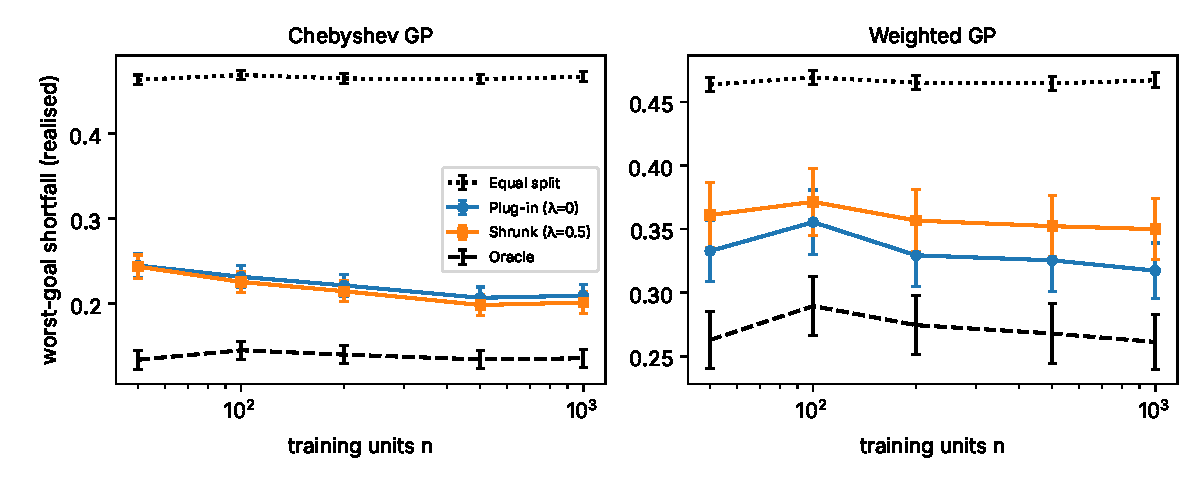
\includegraphics[width=.95\textwidth]{fig_main.pdf}
\caption{Realised worst-goal shortfall against training size (mean with 95\% intervals). Left: Chebyshev GP; right: weighted GP.}\label{fig:main}\end{figure}
\begin{table}[t]\centering\small\begin{tabular}{rlcccc}\toprule
$n$ & Model & Equal & Plug-in & Shrunk ($\lambda{=}0.5$) & Oracle\\\midrule
50 & Chebyshev & 0.464 & 0.245 & 0.244 & 0.134\\
100 & Chebyshev & 0.469 & 0.232 & 0.225 & 0.145\\
200 & Chebyshev & 0.465 & 0.221 & 0.215 & 0.140\\
500 & Chebyshev & 0.465 & 0.207 & 0.198 & 0.134\\
1000 & Chebyshev & 0.467 & 0.209 & 0.201 & 0.136\\
50 & Weighted & 0.464 & 0.333 & 0.361 & 0.263\\
100 & Weighted & 0.469 & 0.356 & 0.371 & 0.290\\
200 & Weighted & 0.465 & 0.329 & 0.357 & 0.275\\
500 & Weighted & 0.465 & 0.325 & 0.352 & 0.268\\
1000 & Weighted & 0.467 & 0.317 & 0.350 & 0.261\\
\bottomrule\end{tabular}
\caption{Mean realised worst-goal shortfall (200 replications) of each allocation, under each GP model.}\label{tab:main}\end{table}

\paragraph{Learning recovers most of the benefit.} Table~\ref{tab:main} shows equal allocation with a worst-goal shortfall near $0.47$ throughout. Plug-in CGP gives $0.245$ at $n=50$ and $0.209$ at $n=1000$, against an oracle of about $0.135$. So learning closes about two thirds of the equal-to-oracle gap at $n=50$ and about three quarters at $n=1000$ (computed from the table values). A gap to the oracle remains because the effects contain unit-level variation that features do not explain. Under WGP, the oracle itself concentrates shortfall on one goal ($0.26$ worst-goal) and plug-in WGP gives $0.33$ to $0.32$, while its mean shortfall is lower than under CGP ($0.13$ to $0.14$ against $0.15$ to $0.16$).

\paragraph{Shrinkage is model-dependent.} Table~\ref{tab:paired} reports paired differences relative to plug-in; negative is better. Under CGP, shrinkage is neutral at small $\lambda$ and harmful at larger $\lambda$ when $n=50$ (worse by $0.009$ at $\lambda=1$ and $0.032$ at $\lambda=1.5$), and helpful at $n=1000$ (better by $0.006$ to $0.011$ for $\lambda\in[0.25,1]$, several standard errors from zero). Under WGP, every $\lambda$ made the worst-goal shortfall \emph{worse}, by roughly $0.02$ to $0.04$. The mean shortfall changes by at most $0.01$ in either direction. A plausible reason, which we did not test, is that weighted-sum GP can sacrifice a goal and shrinkage lowers the attainable level of every goal, which pushes more mass onto the sacrificed one. Chebyshev GP spreads effort across goals.

\begin{table}[t]\centering\small\begin{tabular}{rlccc}\toprule
$n$ & Model & $\lambda{=}0.25$ & $\lambda{=}0.5$ & $\lambda{=}1$\\\midrule
50 & Chebyshev & -0.0026 (0.0014) & -0.0013 (0.0020) & +0.0091 (0.0031)\\
200 & Chebyshev & -0.0044 (0.0010) & -0.0068 (0.0015) & -0.0036 (0.0023)\\
1000 & Chebyshev & -0.0059 (0.0009) & -0.0081 (0.0013) & -0.0105 (0.0021)\\
50 & Weighted & +0.0194 (0.0034) & +0.0283 (0.0047) & +0.0376 (0.0062)\\
200 & Weighted & +0.0145 (0.0033) & +0.0273 (0.0044) & +0.0319 (0.0049)\\
1000 & Weighted & +0.0168 (0.0032) & +0.0326 (0.0045) & +0.0394 (0.0055)\\
\bottomrule\end{tabular}
\caption{Paired change in worst-goal shortfall relative to plug-in (standard error in parentheses). Negative values favour shrinkage.}\label{tab:paired}\end{table}
\begin{table}[t]\centering\small\begin{tabular}{llrcccc}\toprule
Scenario & Model & $n$ & Equal & Plug-in & Shrunk & Oracle\\\midrule
$\tau{=}0.1$ & Chebyshev & 100 & 0.462 & 0.203 & 0.197 & 0.149\\
$\tau{=}0.1$ & Chebyshev & 500 & 0.463 & 0.178 & 0.171 & 0.146\\
$\tau{=}0.6$ & Chebyshev & 100 & 0.481 & 0.318 & 0.312 & 0.143\\
$\tau{=}0.6$ & Chebyshev & 500 & 0.482 & 0.286 & 0.276 & 0.146\\
$\sigma{=}0.1$ & Chebyshev & 100 & 0.467 & 0.235 & 0.231 & 0.145\\
$\sigma{=}0.1$ & Chebyshev & 500 & 0.467 & 0.209 & 0.202 & 0.144\\
$\sigma{=}0.8$ & Chebyshev & 100 & 0.467 & 0.268 & 0.263 & 0.145\\
$\sigma{=}0.8$ & Chebyshev & 500 & 0.467 & 0.225 & 0.223 & 0.144\\
\bottomrule\end{tabular}
\caption{Sensitivity to unit-level noise $\tau$ and measurement noise $\sigma$ under CGP (100 replications). Worst-goal shortfall.}\label{tab:sens}\end{table}

\paragraph{Sensitivity.} Table~\ref{tab:sens} shows the same ordering when $\tau$ or $\sigma$ changes. Larger idiosyncratic noise $\tau$ widens the oracle gap most (plug-in $0.286$ at $\tau=0.6$, $n=500$, against $0.178$ at $\tau=0.1$). Under CGP, shrunk GP with $\lambda=0.5$ is slightly better than plug-in in all eight sensitivity cells, by $0.002$ to $0.010$; we did not compute standard errors for these cells, so they are indicative only.

\paragraph{Optimism.} We also recorded the gap between realised and model-predicted worst-goal shortfall for plug-in GP. Under CGP the realised value exceeded the predicted one by $0.020$ at $n=50$ and $0.001$ at $n=1000$, which is consistent with the optimizer's curse and fades with data. Under WGP the sign was reversed, so this diagnostic does not support a general claim of optimism.

\section{Discussion and limitations}
The results support three practical points. A learned GP is much better than a rule of thumb. The remaining gap to the oracle is driven mainly by unexplained unit-level variation, which more training data cannot remove. And uncertainty adjustments should be tuned to the GP variant, since the adjustment that helps Chebyshev GP hurt weighted GP here.

Limitations are substantial. All data are synthetic, with linear effects and no interactions between units, so the numbers do not describe any real budget. Aspiration levels are exogenous; we do not model their elicitation or learning, nor lexicographic GP. We evaluated fixed values of $\lambda$ rather than a data-driven choice, which a decision maker would need. Only ridge regression was used; nonlinear learners and decision-focused training \citep{elmachtoub2022} are natural extensions. Sensitivity runs are smaller than the main runs and one random-number stream per configuration was used. Applying the method to real regional data, with a validated effect model, remains to be done.

\section{Conclusion}
Predict-then-optimize goal programming with learned marginal effects substantially outperforms equal allocation in simulation. Shrinking predictions by cross-validated residual scale helps Chebyshev GP at larger sample sizes, is marginal at small ones, and hurts the worst-goal shortfall of weighted GP. We recommend treating the adjustment as a tunable robustness device rather than a default.

\paragraph{Reproducibility.} Simulation code (\texttt{code/gp\_ml.py}), the report script (\texttt{code/make\_report.py}) and raw results (\texttt{results/results.json}) accompany this manuscript.

\bibliographystyle{plainnat}
\bibliography{refs}
\end{document}
